\section{Sombreado de Vóxeles} % (fold)
\label{sec:sombreado_de_voxeles}
Para el cálculo de iluminación indirecta es necesario sombrear cada vóxel. El proceso de sombreado de vóxeles nos permite almacenar la radiancia incidente sobre la escena discretizada en vóxeles. En el trabajo de Crassin esto se hace calculando la iluminación directa sobre los vóxeles utilizando \emph{light-view maps} por cada fuente de luz como ya fue explicado en la sección \ref{subsub:voxel_capture}. Este proceso puede ser ineficiente tanto en consumo de memoria como en rendimiento cuando se considera una escena con muchas luces ya que por cada luz se debe realizar este proceso y se debe tener un mapa de luz-vista asociado (seis para luces puntuales). Otra desventaja de este método es la dependencia del rendimiento con la resolución del mapa de luz-vista. Al aumentar la resolución de esta textura también se aumenta el número de colisiones por cada fragmento que desear escribir sobre un mismo vóxel.

Nuestra implementación utiliza \emph{compute shaders} o el procesador de computo en la \ac{GPU} para el sombreado difuso de cada vóxel. Para calcular el termino difuso sobre un fragmento utilizando la \ac{BRDF} de Lambert (ecuación \ref{eq:lambert}) necesitamos saber el valor de $\rho_{d}$ el cual ya es almacenado en nuestro volumen albedo. Esta constante luego debe ser multiplicada por el $\cos(N_{x}, \Psi)$ o atenuación normal. Por esto también se crea un volumen de normales. El vector $\Psi$ se obtiene a partir la dirección de cada fuente de luz en escena.

Para fuentes de luz con dirección no uniforme como luces puntuales o focales es además necesario saber la posición de este fragmento. Siendo cada vóxel una representación discreta de un espacio en escena almacenado en una textura 3D, esta posición se extrae fácilmente convirtiendo la posición tridimensional del vóxel en espacio textura a su equivalente en espacio de mundo.

Al promediar las normales en el espacio de un vóxel pueden surgir varios problemas de precisión. Esto sucede especialmente cuando un vóxel envuelve superficies finas cercanas con normales disparejas. Para solventar este problema se implementaron dos modelos de iluminación de vóxeles. El modelo de Lambert clásico utilizando la normal promedio del vóxel directamente y otro modelo al cual llamaremos Lambert direccional ponderado donde se calcula la atenuación normal por cada cara del vóxel para luego promediar este resultado según el peso de cada eje en el vector normal promedio.

\begin{figure}[H]
	\centering
	\begin{subfigure}[t]{0.33\textwidth}
		\centering
		\captionsetup{justification=centering}
		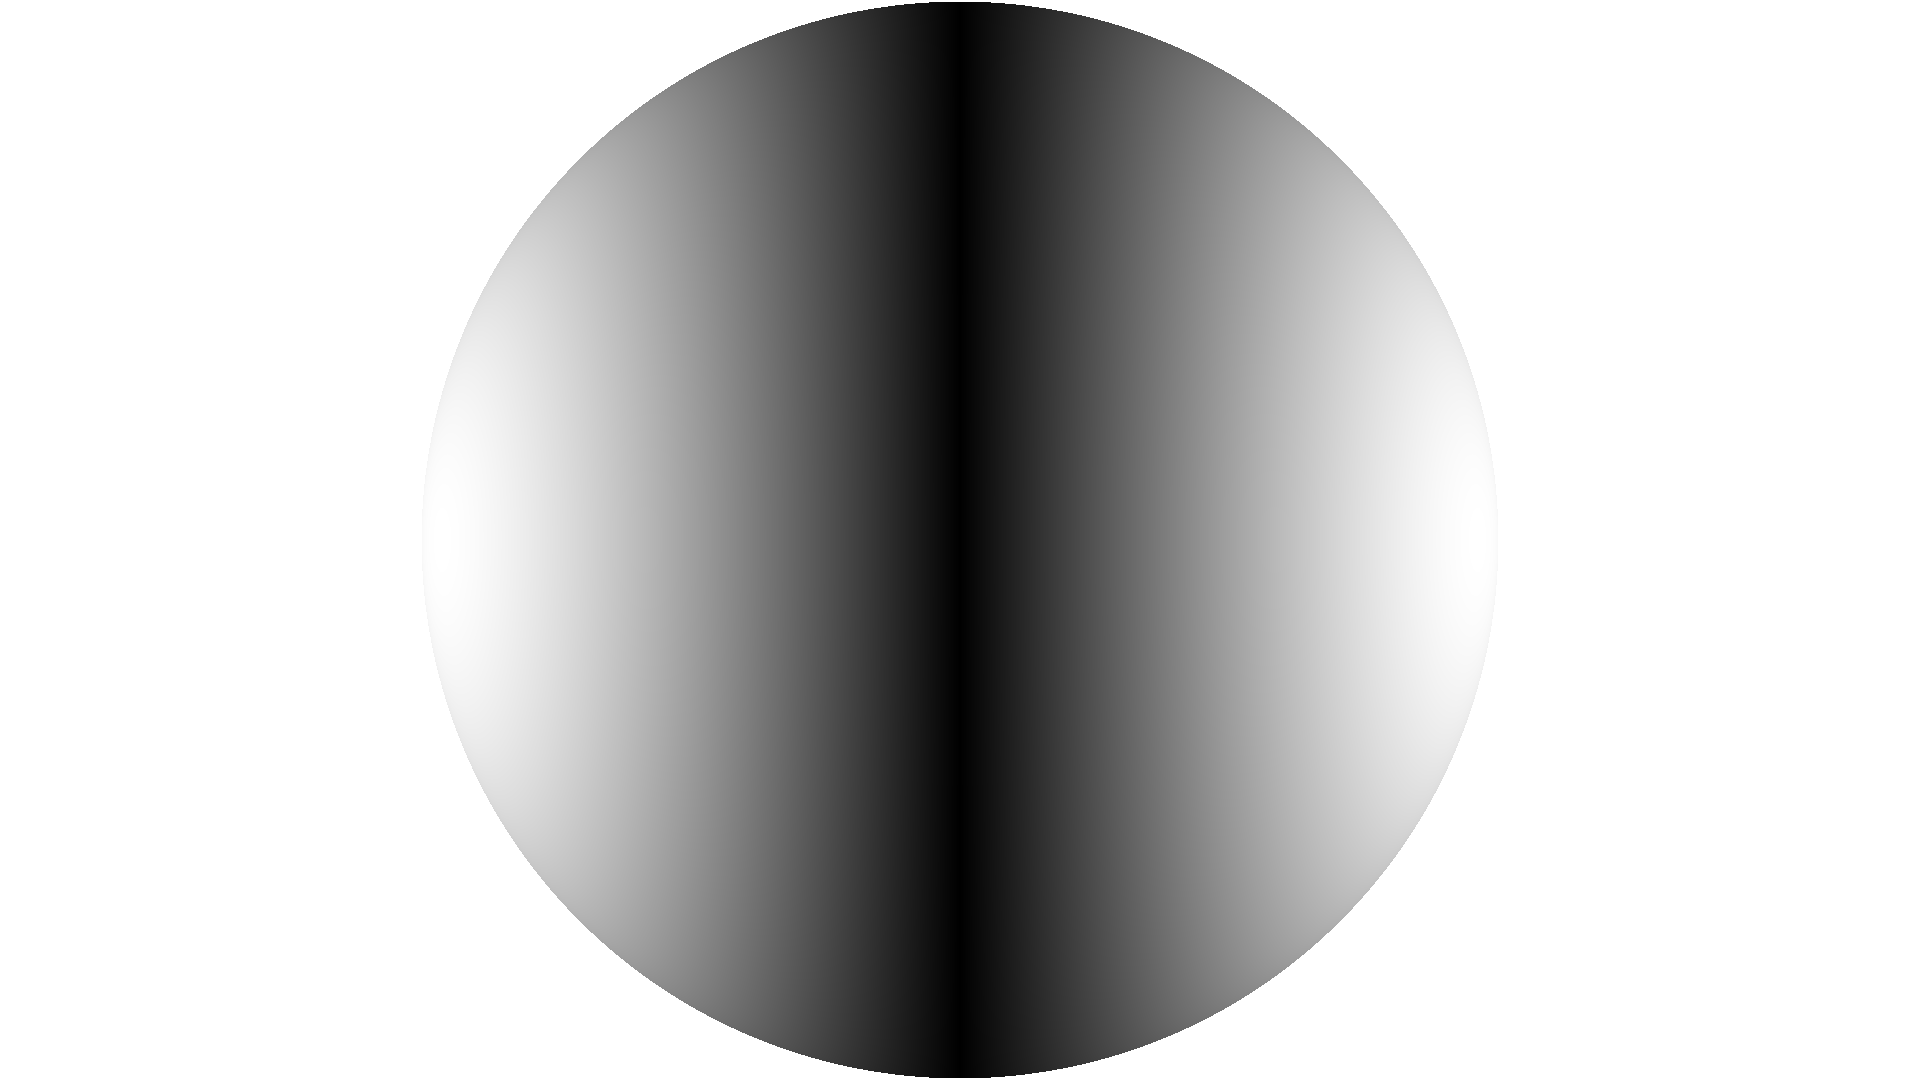
\includegraphics[width=\linewidth]{media/lambert_right.png}
		\caption*{Eje x.}
	\end{subfigure}%
	\begin{subfigure}[t]{0.33\textwidth}
		\centering
		\captionsetup{justification=centering}
		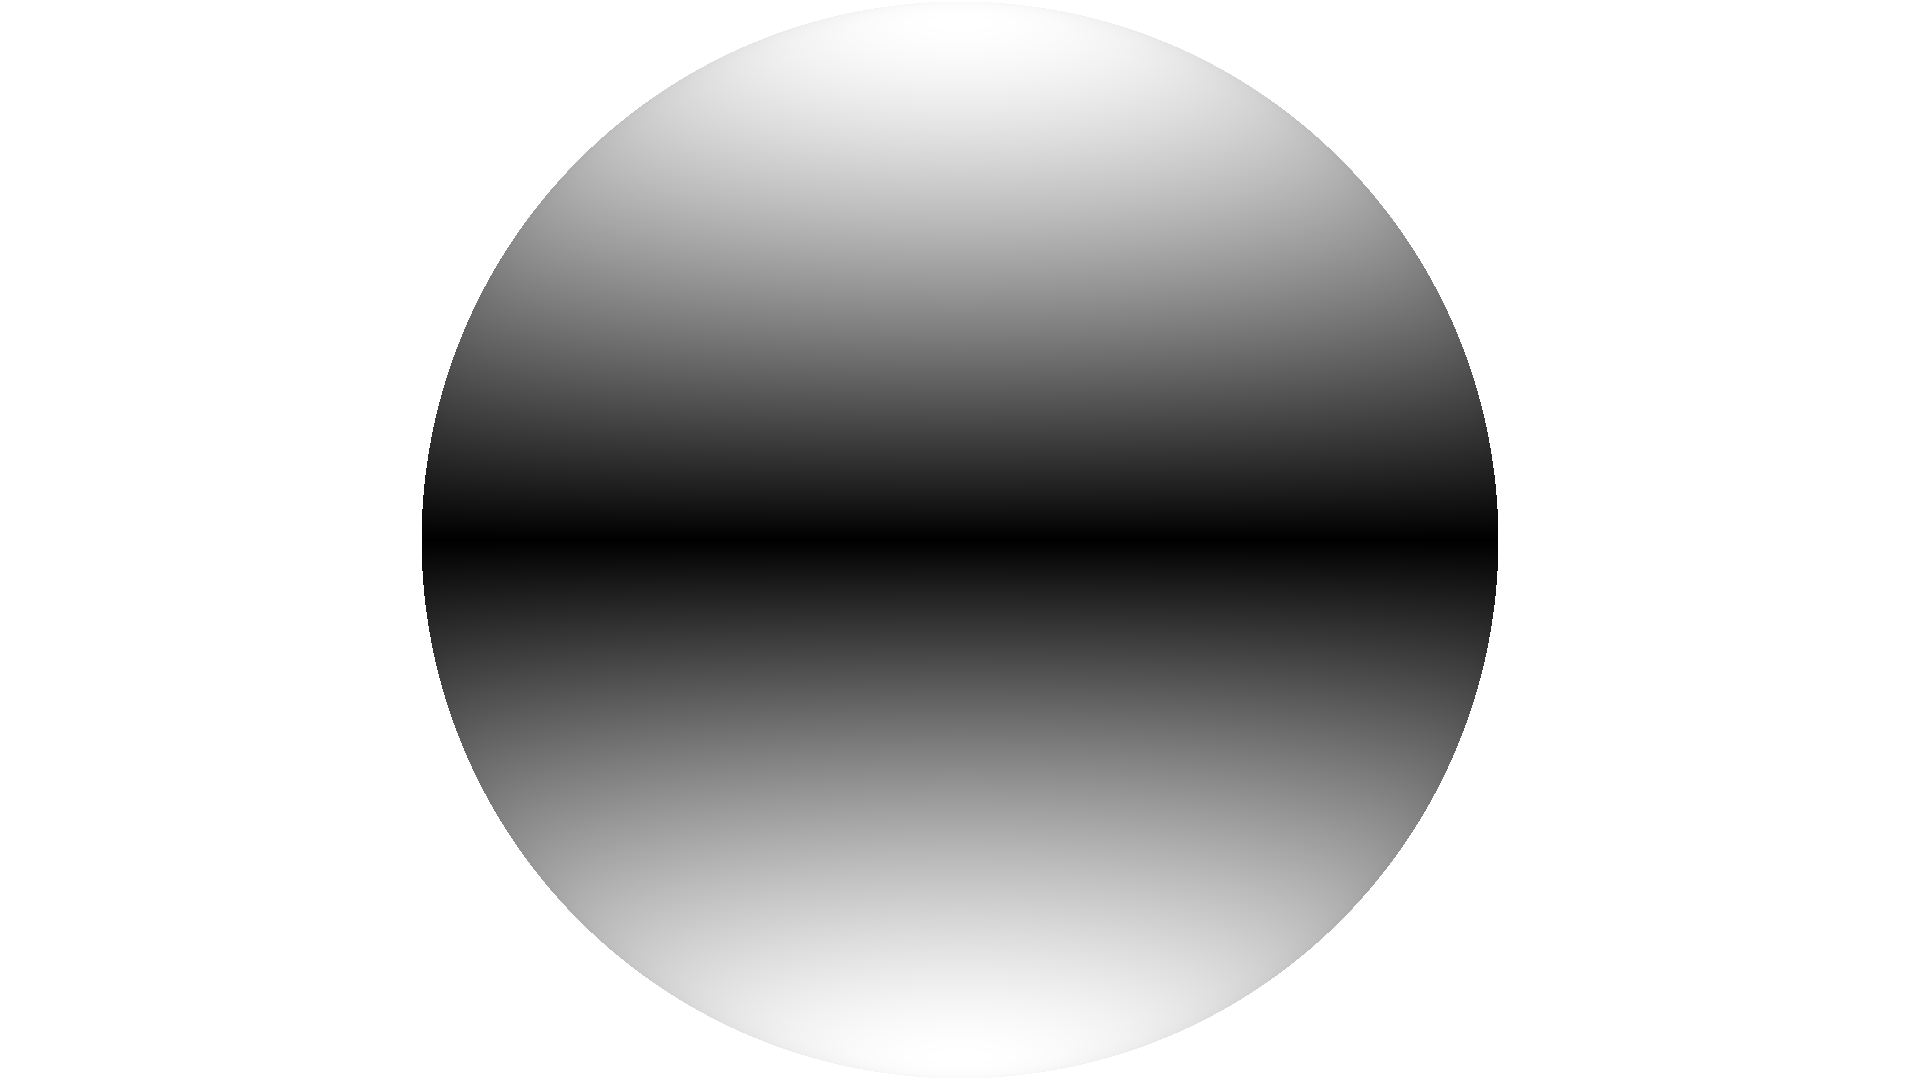
\includegraphics[width=\linewidth]{media/lambert_up.png}
		\caption*{Eje y.}
	\end{subfigure}%
	\begin{subfigure}[t]{0.33\textwidth}
		\centering
		\captionsetup{justification=centering}
		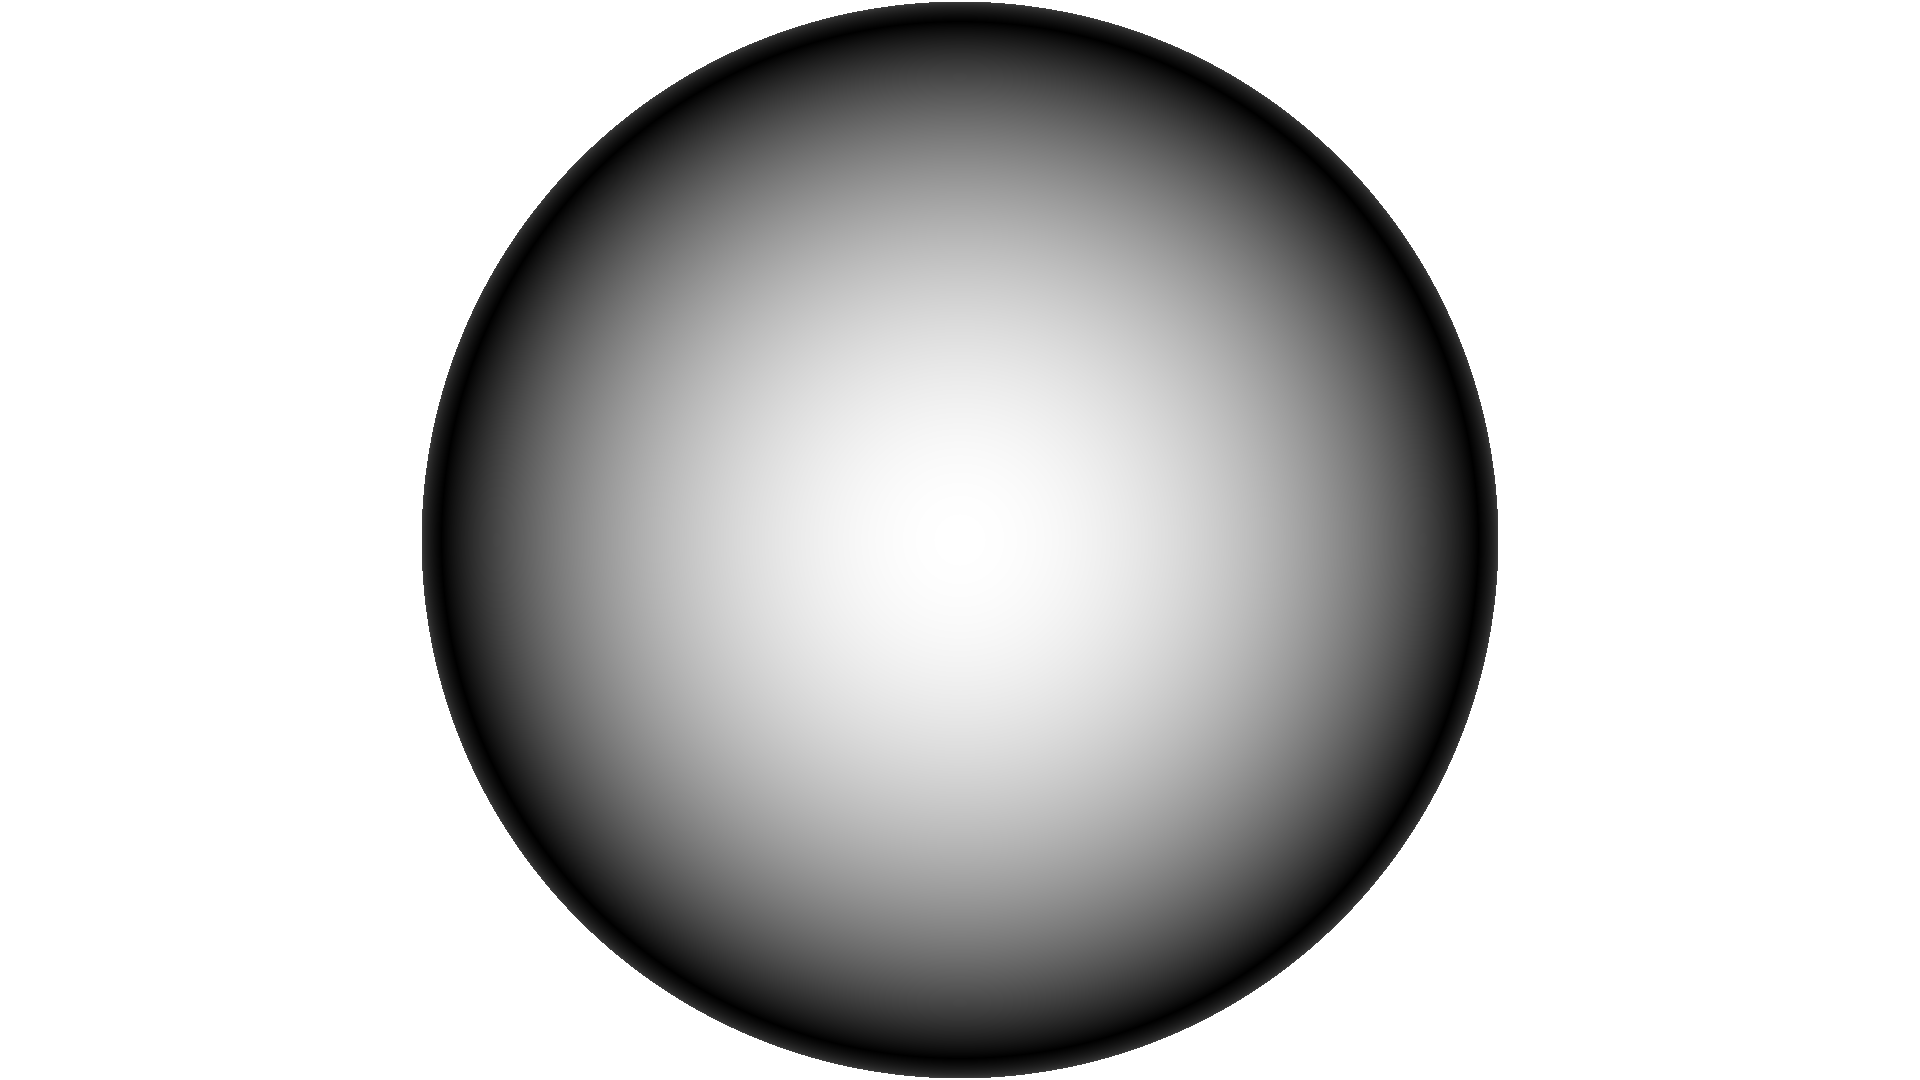
\includegraphics[width=\linewidth]{media/lambert_forward.png}
		\caption*{Eje z.}
	\end{subfigure}%
	\caption{Ilustración de sombreado por cada eje direccional para las caras del vóxel.}
	\label{fig:lambert_dir}
\end{figure}
% section sombreado_de_voxeles (end)

\begin{figure}[H]
	\centering
	\begin{subfigure}[t]{0.49\textwidth}
		\centering
		\captionsetup{justification=centering}
		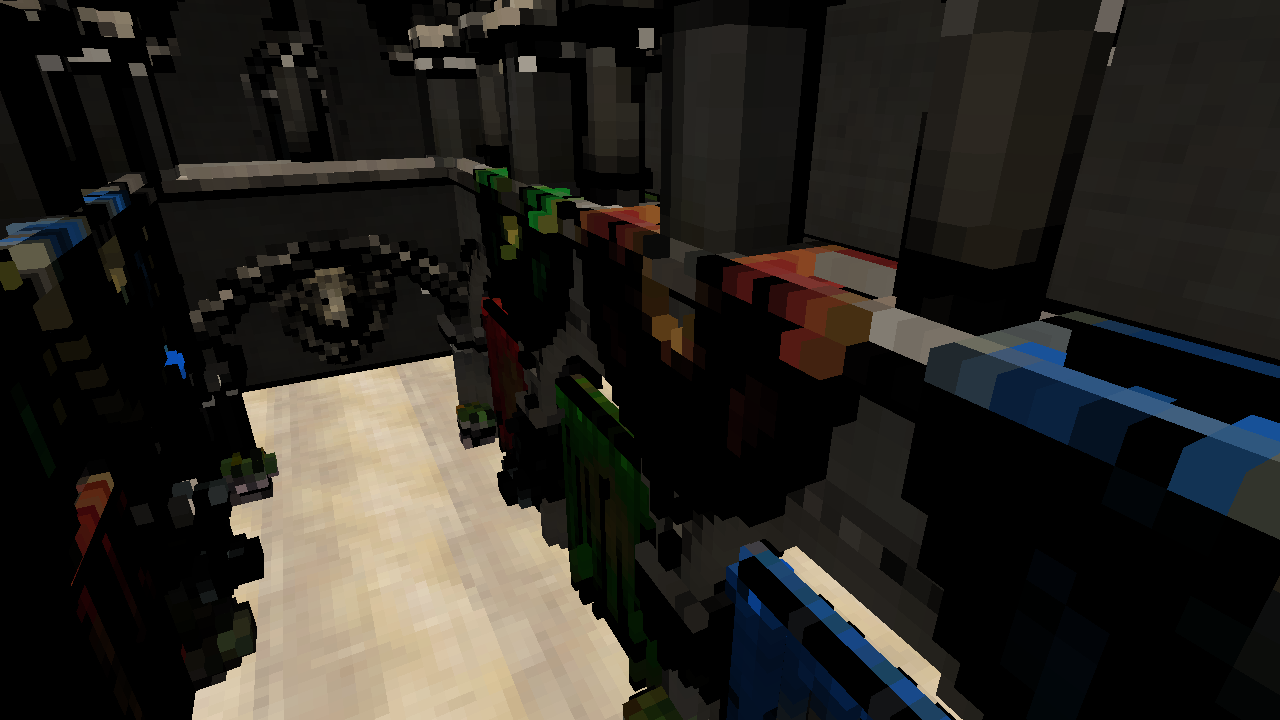
\includegraphics[width=\linewidth]{media/classic_lambert.png}
		\caption*{Lambert.}
	\end{subfigure}%
	\hspace{0.01\textwidth}
	\begin{subfigure}[t]{0.49\textwidth}
		\centering
		\captionsetup{justification=centering}
		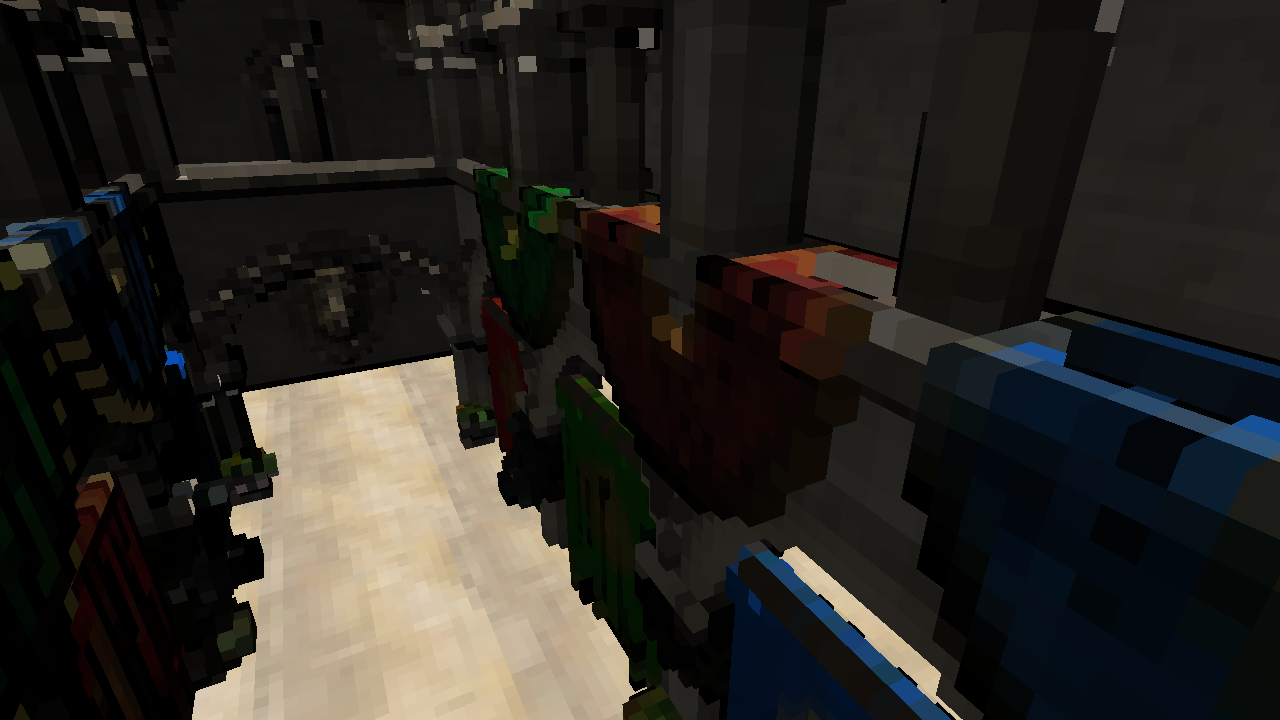
\includegraphics[width=\linewidth]{media/dir_lambert.png}
		\caption*{Lambert direccional ponderado.}
	\end{subfigure}%
	\caption{Sombreado difuso de vóxeles utilizando Lambert clásico y Lambert direccional ponderado. En la imagen izquierda se puede observar varios vóxeles totalmente negros, estos valores son incorrectos, causados por normales desviadas durante el proceso de voxelización. En la imagen derecha estos vóxeles ahora tienen coloración correcta. También se puede observar que objetos con normales promediadas correctamente como el piso mantienen su sombreado original en ambos modelos.}
	\label{fig:lambert_dir_diff}
\end{figure}

\subsection{Trazado y Mapeo de Sombras sobre el Volumen} % (fold)
\label{sub:trazado_de_sombras_sobre_el_volumen}

Para obtener resultados coherentes durante el trazado de conos es también necesario ocluir los vóxeles con sombras generadas a partir de distintas fuentes de luz en escena. Utilizando mapas de luz-vista como en el trabajo de Crassin esto es sencillo ya que los vóxeles ocluidos simplemente no reciben fotones durante el proceso de captura de la iluminación directa (sección \ref{subsub:voxel_capture}).

\begin{figure}[H]
	\centering
	\begin{subfigure}[t]{0.49\textwidth}
		\centering
		\captionsetup{justification=centering}
		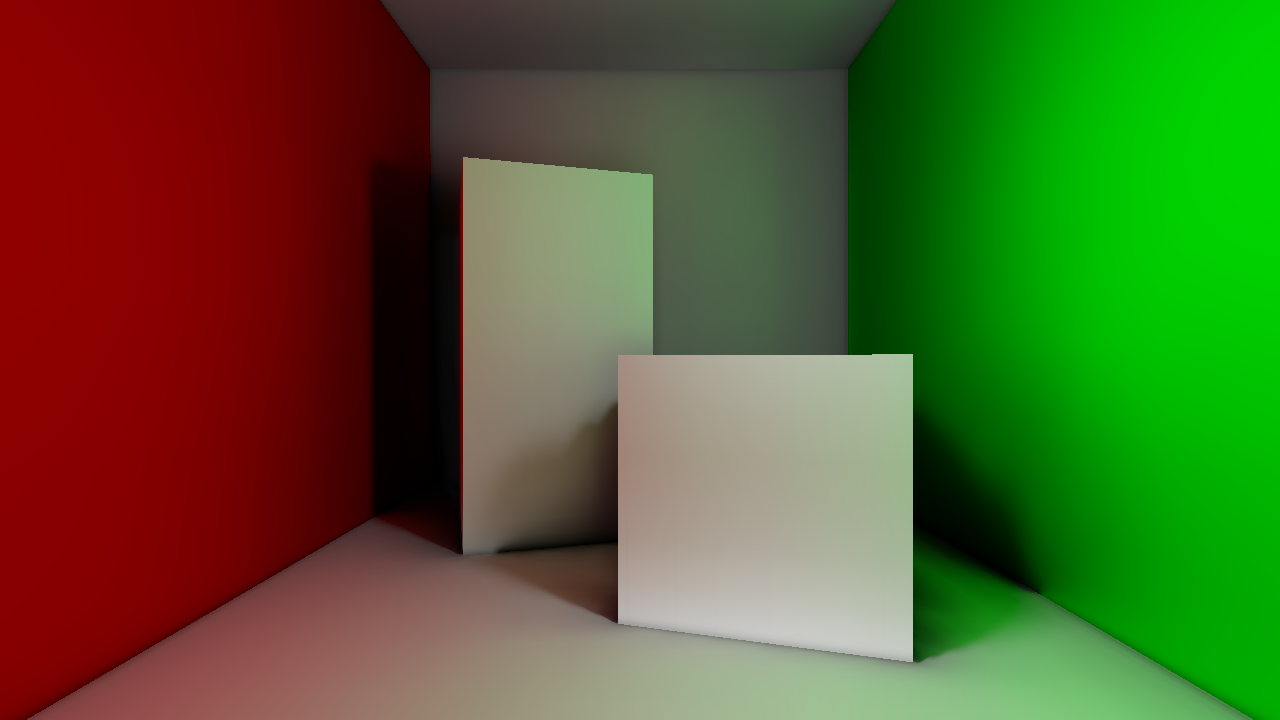
\includegraphics[width=\linewidth]{media/voxel_shadowing.png}
		\caption*{Con vóxeles ocluidos por sombras.}
	\end{subfigure}%
	\hspace{0.01\textwidth}
	\begin{subfigure}[t]{0.49\textwidth}
		\centering
		\captionsetup{justification=centering}
		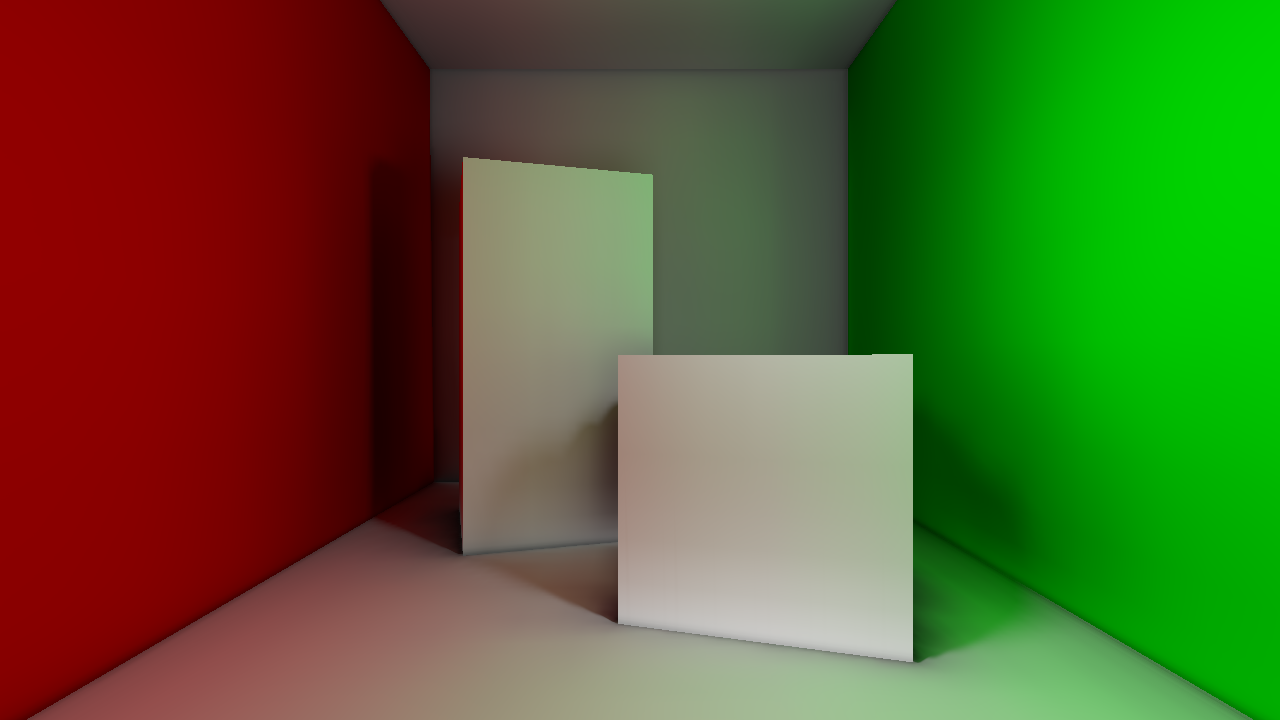
\includegraphics[width=\linewidth]{media/voxel_noshadowing.png}
		\caption*{Sin oclusión de vóxeles.}
	\end{subfigure}%
	\caption{Iluminación global incorrecta al utilizar una representación con vóxeles sin oclusión.}
	\label{fig:voxel_shadow_error}
\end{figure}

En nuestra implementación existen distintas opciones para trazar sobras sobre los vóxeles. Este proceso se realiza durante el sombreado de vóxeles explicado anteriormente.

Para luces directas se utiliza mapeo de sombras visto en la sección \ref{subsec:shadowmapping}. En  esta técnica es necesario obtener la posición en espacio de mundo del vóxel. Para esto la posición tridimensional del vóxel en espacio de textura se transforma a espacio de mundo. De esta transformación se obtiene la posición central del vóxel. Utilizar el centro del vóxel para mapeo de sombras puede ocasionar problemas cuando este punto esta ocluido por otras superficies dentro del mismo vóxel o fragmentos cercanos ya que el mapa de sombras es una representación mucho más detallada de la escena vista desde una fuente de luz. Para solventar este problema se traslada la posición del vóxel según la normal por el tamaño medio de un vóxel.

Estando el mapeo de sombras solo disponible en nuestra implementación para solo una luz directa se implementó trazado de sombras para cualquier fuente de luz puntual, focal o direccional. Los volúmenes resultantes del proceso de voxelización puede ser utilizado para trazar rayos sobre la escena discretizada. Siendo estos volúmenes una representación mucho más simple de la escena original, utilizar técnicas de comunes en trazado de rayos (sección \ref{subsec:monte_carlo_raytracing}) es viable.

Para realizar pruebas de oclusión sobre un vóxel por una fuente de luz se lanza un rayo desde la posición del vóxel en la dirección opuesta de la luz incidente. Si este rayo colisiona con otro vóxel entonces el vóxel original esta ocluido.

\subsubsection{Trazado de Sombras Suaves sobre el Volumen}

Una técnica que incrementa la calidad visual de las sombras es la generación de un bordeado suave para las sombras. En trazado de rayos esto se logra lanzando varios rayos en distintas direcciones en vez de uno solo para generar varias muestras de oclusión.

\begin{figure}[H]
	\centering
	\begin{subfigure}[t]{0.49\textwidth}
		\centering
		\captionsetup{justification=centering}
		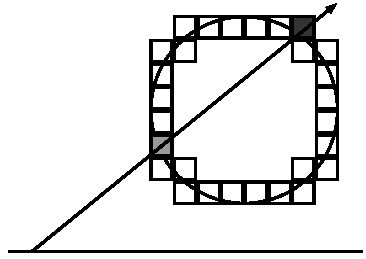
\includegraphics[width=\linewidth]{media/shadow_tracer.pdf}
		\caption*{Rayo alejado de los bordes de la superficie.}
	\end{subfigure}%
	\hspace{0.01\textwidth}
	\begin{subfigure}[t]{0.49\textwidth}
		\centering
		\captionsetup{justification=centering}
		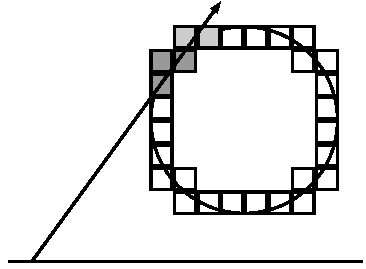
\includegraphics[width=\linewidth]{media/shadow_trace_corner.pdf}
		\caption*{Rayo cercano al el borde de la superficie.}
	\end{subfigure}%
	\caption{Descripción grafica del proceso de acumulación de colisiones a través del recorrido de un rayo para prueba de oclusión.}
	\label{fig:soft_voxel_shadow}
\end{figure}

En nuestra implementación logramos obtener bordes suaves para las sombras generadas durante el sombreado de vóxeles con un solo rayo. Esta técnica se basa en el hecho de que al trazar un rayo hacia una superficie voxelizada este rayo chocara más veces contra vóxeles cerca de los bordes de la superficie vistos desde la fuente de luz. Como se observa en la figure \ref{fig:soft_voxel_shadow} en vez de detener el rayo una vez que se ha encontrado una colisión ahora se le asigna un valor a cada colisión y se ve acumulando este factor a través del recorrido del rayo dividido por la distancia recorrida.


% subsection trazado_de_sombras_sobre_el_volumen (end)
